\documentclass{article}
\usepackage{tikz}
\usetikzlibrary{arrows.meta,positioning,calc,shapes.geometric}
\pagestyle{empty}
\begin{document}
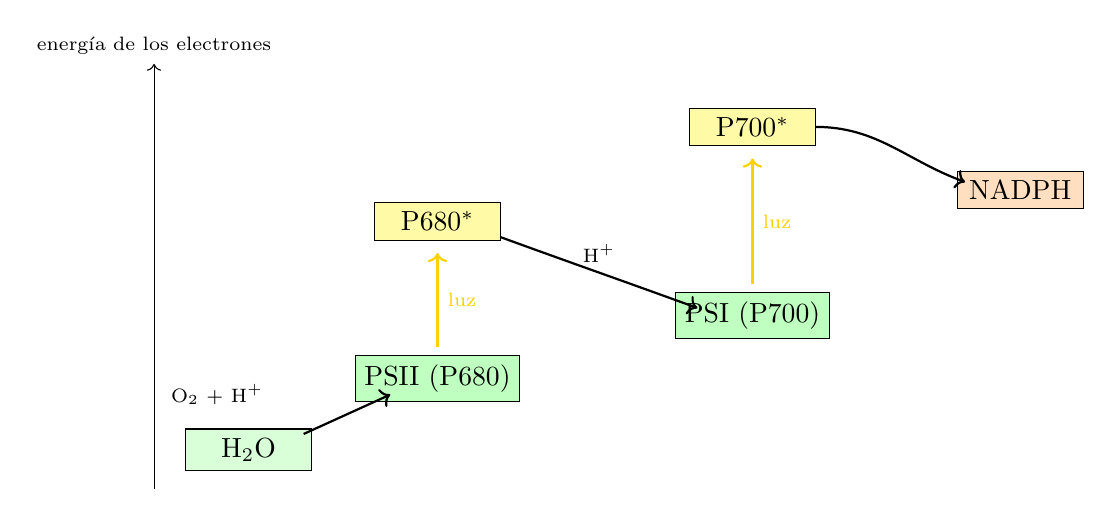
\begin{tikzpicture}

\draw[->] (0,0) -- (0,5.4) node[above, font=\scriptsize] {energía de los electrones};
\node[draw, fill=green!15, minimum width=1.6cm] (h2o) at (1.2,0.5) {H$_2$O}; \node[draw, fill=green!25, minimum width=1.6cm] (p2) at (3.6,1.4) {PSII (P680)}; \node[draw, fill=yellow!35, minimum width=1.6cm] (p2x) at (3.6,3.4) {P680$^*$};
\node[draw, fill=green!25, minimum width=1.6cm] (p1) at (7.6,2.2) {PSI (P700)}; \node[draw, fill=yellow!35, minimum width=1.6cm] (p1x) at (7.6,4.6) {P700$^*$};
\node[draw, fill=orange!25, minimum width=1.6cm] (nadph) at (11.0,3.8) {NADPH};
\draw[->, thick, yellow!70!orange] (3.6,1.8) -- (3.6,3.0) node[midway, right, font=\scriptsize] {luz};
\draw[->, thick, yellow!70!orange] (7.6,2.6) -- (7.6,4.2) node[midway, right, font=\scriptsize] {luz};
\draw[->, thick] (1.9,0.7) -- (3.0,1.2); \node[font=\scriptsize] at (0.8,1.2) {O$_2$ + H$^+$};
\draw[->, thick] (4.4,3.2) to[out=-20, in=160] node[midway, above, font=\scriptsize] {H$^+$} (6.9,2.3);
\draw[->, thick] (8.4,4.6) to[out=0, in=160] (10.3,3.9);

\end{tikzpicture}
\end{document}
